\documentclass[tikz, border=20pt]{standalone}
\usepackage{amsmath}
\usetikzlibrary{arrows.meta, calc, positioning, shapes.geometric, fit, backgrounds}

\definecolor{pnavy}{HTML}{0E2A47}
\definecolor{pteal}{HTML}{356170}
\definecolor{pgold}{HTML}{B5842A}
\definecolor{pgrey}{HTML}{495057}
\definecolor{plight}{HTML}{F8F9FA}
\definecolor{preject}{HTML}{8C2F39}

\begin{document}
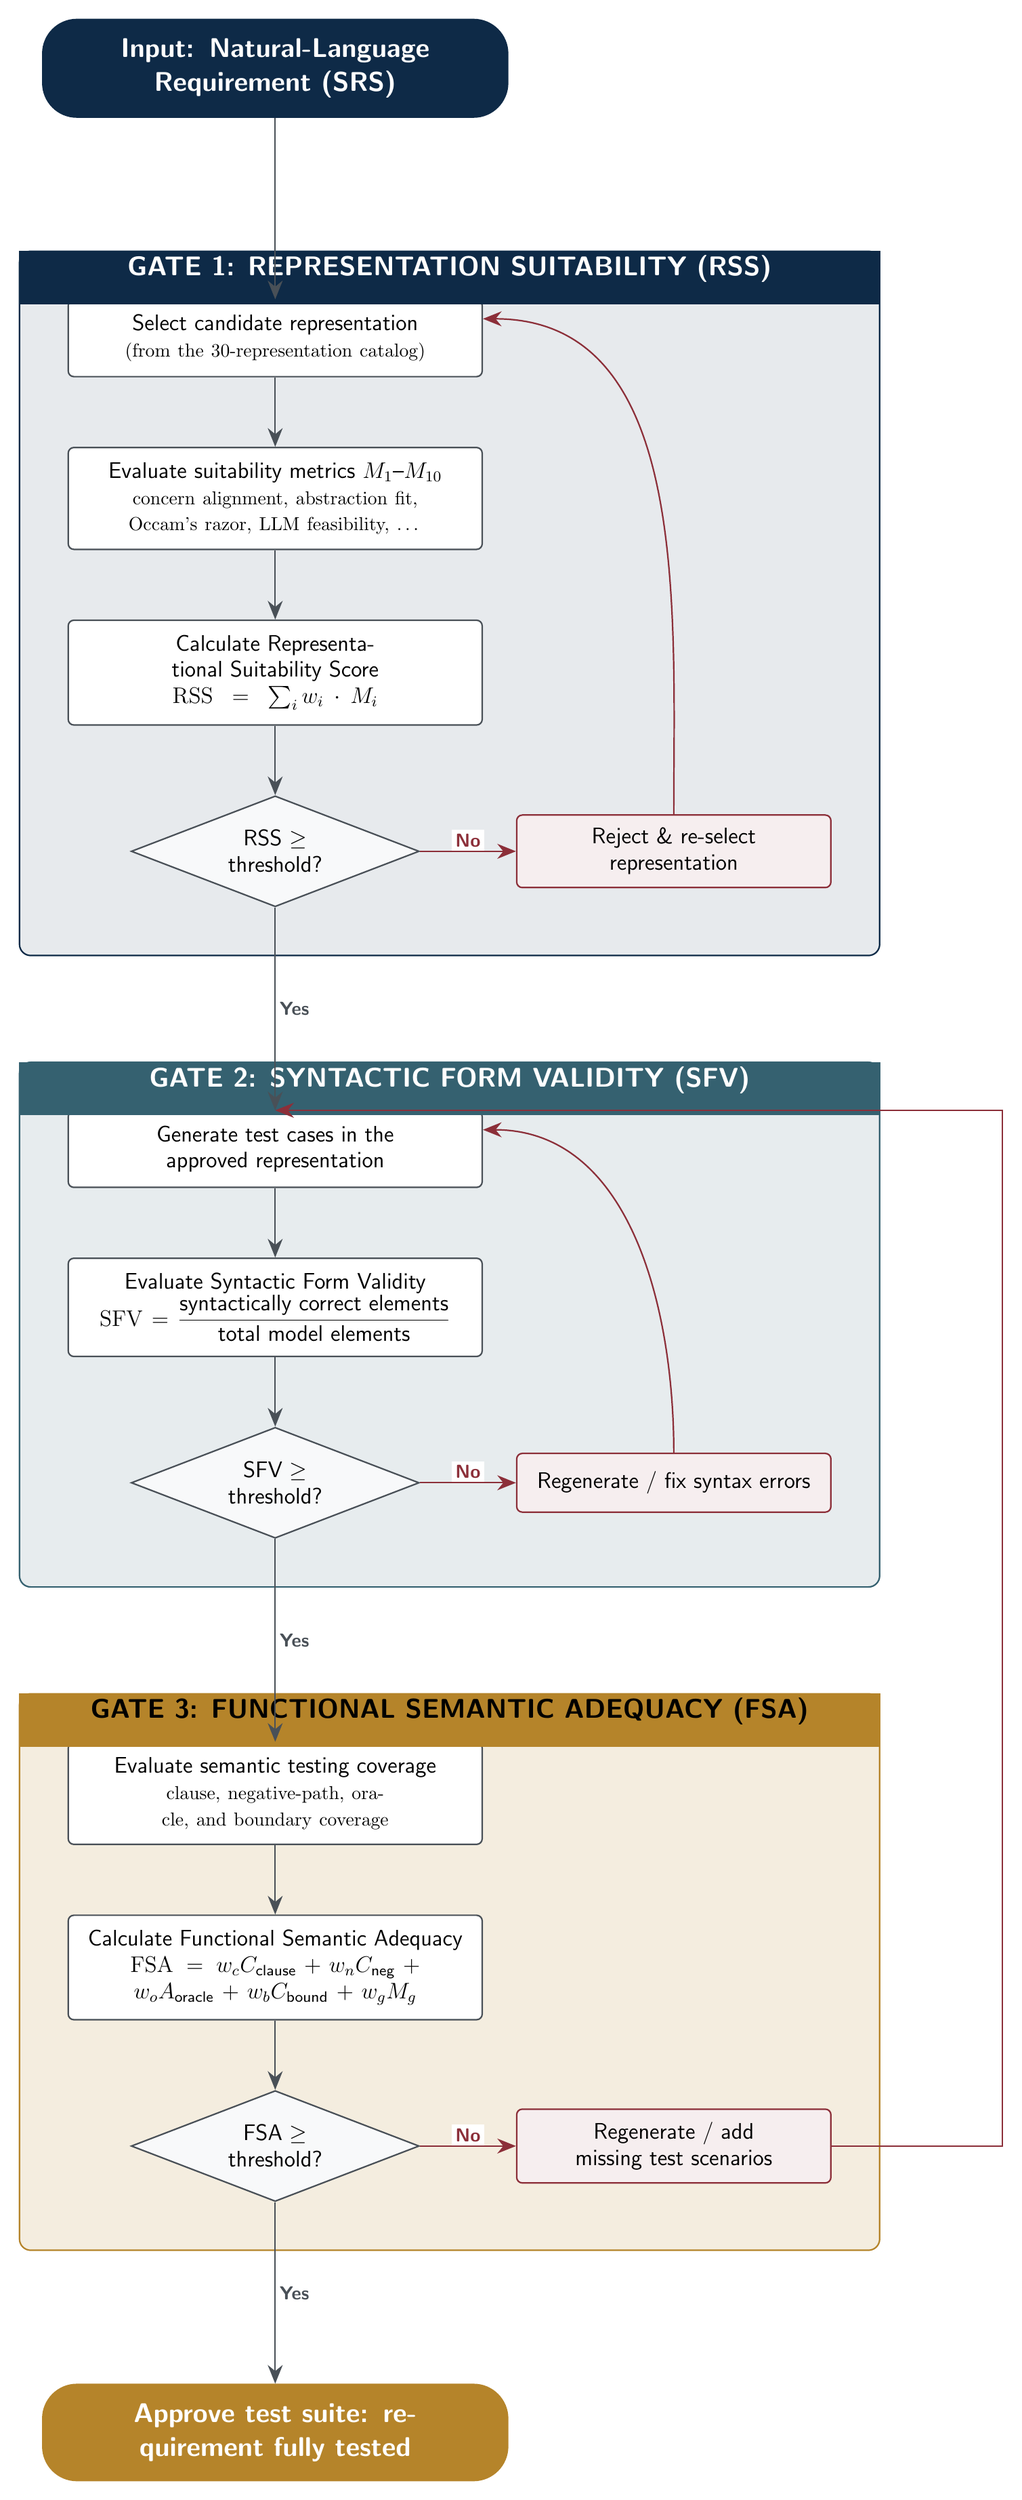
\begin{tikzpicture}[
  font=\sffamily,
  procbox/.style={rectangle, rounded corners=3pt, draw=pgrey, thick, fill=white,
    text width=7.2cm, align=center, minimum height=1.3cm, inner sep=8pt, font=\sffamily\large},
  decision/.style={diamond, draw=pgrey, thick, fill=plight, aspect=2.6,
    text width=2.6cm, align=center, inner sep=3pt, font=\sffamily\large},
  reject/.style={rectangle, rounded corners=3pt, draw=preject, thick, fill=preject!8,
    text width=5.4cm, align=center, minimum height=1.1cm, inner sep=7pt, font=\sffamily\large},
  endpoint/.style={rectangle, rounded corners=18pt, draw=pnavy, very thick, fill=pnavy,
    text=white, text width=8cm, align=center, minimum height=1.3cm, inner sep=10pt, font=\sffamily\Large\bfseries},
  titlebar/.style={font=\sffamily\Large\bfseries, text=white, align=center},
  arr/.style={-{Stealth[length=3.5mm, width=2.8mm]}, thick, pgrey},
  rejarr/.style={-{Stealth[length=3.5mm, width=2.8mm]}, thick, preject},
  yeslabel/.style={font=\sffamily\bfseries\normalsize, fill=white, inner sep=2pt},
  nolabel/.style={font=\sffamily\bfseries\normalsize, text=preject, fill=white, inner sep=2pt},
  node distance=13mm and 18mm
]

% ================= NODES =================
\node[endpoint] (start) {Input: Natural-Language Requirement (SRS)};

% ---- Gate 1 nodes ----
\node[procbox, below=34mm of start] (a1) {Select candidate representation\\\textnormal{\normalsize (from the 30-representation catalog)}};
\node[procbox, below=of a1] (a2) {Evaluate suitability metrics $M_1$--$M_{10}$\\\textnormal{\normalsize concern alignment, abstraction fit, Occam's razor, LLM feasibility, \ldots}};
\node[procbox, below=of a2] (a3) {Calculate Representational Suitability Score\\$\displaystyle\mathrm{RSS} = \textstyle\sum_i w_i \cdot M_i$};
\node[decision, below=of a3] (a4) {RSS $\geq$\\threshold?};
\node[reject, right=of a4] (a5) {Reject \& re-select representation};

% ---- Gate 2 nodes ----
\node[procbox, below=38mm of a4] (b1) {Generate test cases in the approved representation};
\node[procbox, below=of b1] (b2) {Evaluate Syntactic Form Validity\\$\mathrm{SFV} = \dfrac{\text{syntactically correct elements}}{\text{total model elements}}$};
\node[decision, below=of b2] (b3) {SFV $\geq$\\threshold?};
\node[reject, right=of b3] (b4) {Regenerate / fix syntax errors};

% ---- Gate 3 nodes ----
\node[procbox, below=38mm of b3] (c1) {Evaluate semantic testing coverage\\\textnormal{\normalsize clause, negative-path, oracle, and boundary coverage}};
\node[procbox, below=of c1] (c2) {Calculate Functional Semantic Adequacy\\$\mathrm{FSA} = w_c C_{\text{clause}} + w_n C_{\text{neg}} + w_o A_{\text{oracle}} + w_b C_{\text{bound}} + w_g M_g$};
\node[decision, below=of c2] (c3) {FSA $\geq$\\threshold?};
\node[reject, right=of c3] (c4) {Regenerate / add missing test scenarios};

\node[endpoint, below=34mm of c3, fill=pgold, draw=pgold] (success) {Approve test suite: requirement fully tested};

% ================= PHASE BACKGROUND BOXES =================
\begin{scope}[on background layer]
\node[fit=(a1)(a2)(a3)(a4)(a5), inner sep=9mm, fill=pnavy!10, rounded corners=6pt, draw=pnavy, thick] (phase1box) {};
\node[fit=(b1)(b2)(b3)(b4), inner sep=9mm, fill=pteal!12, rounded corners=6pt, draw=pteal, thick] (phase2box) {};
\node[fit=(c1)(c2)(c3)(c4), inner sep=9mm, fill=pgold!15, rounded corners=6pt, draw=pgold, thick] (phase3box) {};
\end{scope}

% title bars sit fully inside each box, flush with its top edge (no protrusion),
% spanning exactly the box's own width via fit
\node[titlebar, fit=(phase1box.north west)(phase1box.north east), minimum height=10mm,
  fill=pnavy, anchor=north, yshift=0mm, inner sep=0pt] (title1) at (phase1box.north) {GATE 1: REPRESENTATION SUITABILITY (RSS)};
\node[titlebar, fit=(phase2box.north west)(phase2box.north east), minimum height=10mm,
  fill=pteal, anchor=north, yshift=0mm, inner sep=0pt] (title2) at (phase2box.north) {GATE 2: SYNTACTIC FORM VALIDITY (SFV)};
\node[titlebar, fit=(phase3box.north west)(phase3box.north east), minimum height=10mm,
  fill=pgold, text=black, anchor=north, yshift=0mm, inner sep=0pt] (title3) at (phase3box.north) {GATE 3: FUNCTIONAL SEMANTIC ADEQUACY (FSA)};

% ================= INTRA-PHASE ARROWS (drawn first, fine to sit under labels) =================
\draw[arr] (a1) -- (a2);
\draw[arr] (a2) -- (a3);
\draw[arr] (a3) -- (a4);
\draw[rejarr] (a4) -- node[nolabel, above]{No} (a5);
\draw[rejarr] (a5.north) to[out=90, in=0] ($(a1.east)!0.5!(a1.north east)$);

\draw[arr] (b1) -- (b2);
\draw[arr] (b2) -- (b3);
\draw[rejarr] (b3) -- node[nolabel, above]{No} (b4);
\draw[rejarr] (b4.north) to[out=90, in=0] ($(b1.east)!0.5!(b1.north east)$);

\draw[arr] (c1) -- (c2);
\draw[arr] (c2) -- (c3);
\draw[rejarr] (c3) -- node[nolabel, above]{No} (c4);

% long reject loop from Gate 3 back to Gate 2's first step: routed along the
% far right margin, clear of every box, drawn last (see below) so it is never
% hidden under a title bar.

% ================= INTER-PHASE ARROWS (drawn LAST so they paint over any title bar) =================
\draw[arr] (start) -- (a1);
\draw[arr] (a4) -- node[yeslabel, right]{Yes} (b1);
\draw[arr] (b3) -- node[yeslabel, right]{Yes} (c1);
\draw[arr] (c3) -- node[yeslabel, right]{Yes} (success);

\coordinate (farright) at ($(c4.east)+(32mm,0)$);
\draw[rejarr] (c4.east) -- (farright)
  -- (farright |- b1.north)
  -- (b1.north);

\end{tikzpicture}
\end{document}
